\chapter{DATASETS}
\label{chapter:dataset_preparation}

In this thesis, we predict the affinity score of drug-target pairs by using heterogeneous networks generated with the existing information of chemicals, proteins, and enriched with additional information extracted from the text representations of these biomolecules.

We compiled several databases in order to use different data types as inputs to our models to learn the distributional representation vectors of molecules. In this chapter we conduct a literature review about the databases, up-to-date statistical data, and the usage of the information.

\section{BindingDB}
BindingDB \cite{gilson2016bindingdb} is an accessible database of drug target interactions and measured binding affinity values. With statistics as of February 2021, it can be listed as follows: It contains 41.328 entries, 8.202 protein targets each with a DOI, and 2.114.159 binding data for 928.022 small molecules. There are 2,823 protein-ligand crystal structures with BindingDB binding affinity measures for proteins with 100\% sequence identity, and 8.263 crystal structures allowing 85\% sequence identity of proteins. 2.077.458 Ki (nM), Kd (nM), IC50 (nM), EC50 (nM) values were compiled from the database within the scope of the thesis. 

To benchmark the performance of graph-based representational learning we use BDB dataset \cite{ozccelik2021chemboost} that is extracted from the BindingDB database. 24.404 binding affinities observed for all pairs of 924 ligand and 480 proteins, measured by the $pK_d$ value (log transformed kinase dissociation constant). The number of ligands with strong binding affinity values is 3428 (i.e., $pK_d \geq 7$) according to literature \cite{he2017simboost}. Figure \ref{fig:bdb} illustrates the distribution of the binding affinity values of proteins - ligand pairs in BDB dataset. 

\begin{figure}
    \centering
        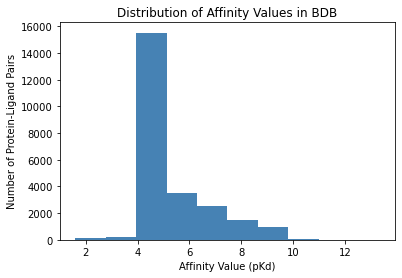
\includegraphics[width=0.5\linewidth]{chapters/datasetpreparation/figures/bdb.png} 
    \caption{Distribution of binding affinity values in BDB.}
    \label{fig:bdb}
\end{figure}

BDB dataset consists of 5 different setups for training and evaluating the model performance. To evaluate the performance of DeepDTA, we trained DeepDTA model with the knowledge derived from heterogeneous networks on five training setups of BDB dataset \cite{ozccelik2021chemboost}, and test the models in the corresponding test sets. 
\section{DrugBank}
DrugBank \cite{wishart2006drugbank, wishart2008drugbank, wishart2018drugbank} is an online database of information about drugs and drug targets. It contains information about drugs, such as chemical, pharmacological, and pharmaceutical data, and information about drug targets, such as sequence, structure, and pathways, as both bioinformatics and cheminformatics sources. Statistical information as of January 2021 is given in Table 
\ref{tab:drugbank_stats}. 14.350 drugs and 2.682.158 drug-drug interaction information from DrugBank were compiled as data within the scope of the project.

\begin{table}[]
\caption{DrugBank statistics (01.2021).}
\centering
\begin{tabular}{|l|l|}
\hline
\multicolumn{1}{|c|}{\textbf{Data}}  & \multicolumn{1}{c|}{\textbf{Number}} \\ \hline
Total Number of Small Molecule Drugs & 11.834                               \\ \hline
Total Number of Biotech Drugs        & 2.481                                \\ \hline
Total Number of Drugs                & 14.315                               \\ \hline
\end{tabular}
\label{tab:drugbank_stats}
\end{table}
\section{SIDER}

SIDER \cite{kuhn2010side, kuhn2016sider} is a database of drugs that have entered the market and their recorded adverse drug reactions extracted from public documents and prospectuses. Information such as side effect frequency, drug and side effect classification, and drug-target relationships are presented in a computer readable format. SIDER uses the Anatomical Therapeutic Chemical (ATC) Classification System, which is a drug classification system that classifies the active substances of drugs according to the organ or system they act on and their therapeutic, pharmacological and chemical properties. Side effects are coded by converting to MedDRA terminology. The current statistics of the data in the database are shown in Table \ref{tab:sider_stats}. From these data, 5,868 side effects and 139,756 drug-side effect relations were compiled within the scope of this thesis.

\begin{table}[]
\caption{SIDER Database statistics (10.2015).}
\centering
\begin{tabular}{|l|l|l|}
\hline
\textbf{Side Effects} & \textbf{Drugs} & \textbf{Drug-Side Effect Pairs} \\ \hline
5.868        & 1.430 & 139.756 \\ \hline
\end{tabular}
\label{tab:sider_stats}
\end{table}
\section{Comparative Toxicogenomics Database}
The Comparative Toxicogenomics Database \cite{davis2021comparative}, CTD, is a database that provides information on manually curated chemical–gene/protein interactions, chemical–disease and gene–disease relationships. CTD has several categories of data. These are chemicals, diseases, chemical-disease relationships, and gene-disease relationships. Statistical data as of February 2021 are given in Table \ref{tab:ctd_stats}. From these data, a total of 2.958.797 chemical-disease relationship and 28.253.189 gene-disease relationship data were compiled within the scope of the project.

\begin{table}[]
\caption{CTD statistics (02.2021).}
\centering
\begin{tabular}{|l|l|}
\hline
\multicolumn{1}{|c|}{\textbf{Data}} & \multicolumn{1}{c|}{\textbf{Number}} \\ \hline
Chemicals                  & 16.572                      \\ \hline
Diseases                   & 7.246                       \\ \hline
Chemical-Disease Relation  & 2.958.797                   \\ \hline
Gene-Disease Relation      & 28.253.189                  \\ \hline
\end{tabular}
\label{tab:ctd_stats}
\end{table}
\section{PubChem}
PubChem is an open chemistry database that contains small molecules, nucleotides, carbohydrates, lipids, peptides, and chemically-modified macromolecules, as well as information on chemical structures, identifiers, chemical and physical properties, biological activities, patents, health, safety, and toxicity data about them. Current statistics in the database are given in Table \ref{tab:pubchem_stats}.

\begin{table}[]
\caption{PubChem statistics (02.2021)}
\centering
\begin{tabular}{|l|l|}
\hline
\multicolumn{1}{|c|}{\textbf{Data}} & \multicolumn{1}{c|}{\textbf{Number}} \\ \hline
Compounds                           & 109.487.163                          \\ \hline
Substances                          & 270.034.522                          \\ \hline
Proteins                            & 96.280                               \\ \hline
Genes                               & 89.655                               \\ \hline
\end{tabular}
\label{tab:pubchem_stats}
\end{table}

 

\section{Universal Protein Resource}
The Universal Protein Source (UniProt) \cite{uniprot2021uniprot}, is an important resource for accessible protein information including protein sequence and functional information. As of June 2021, the total number of entries is 565.254  according to current statistics. 

\section{STRING}
Search Tool for the Retrieval of Interacting Genes/Proteins, STRING \cite{szklarczyk2021string}, is a biological database of known and predicted protein-protein interactions. The interactions include direct (physical) and indirect (functional) associations; they stem from computational prediction, from knowledge transfer between organisms, and from interactions aggregated from other (primary) databases.

The STRING database compiles information from several sources such as computational prediction methods, public text collections, laboratory experiments, and other databases. According to the statistics provided as of August 2021, the STRING database contains 67.592.464 proteins and 296.567.750 interactions at highest security (score $>=$ 0.900),  834.790.438 interactions with high security or better (score $>=$ 0.700), medium security or better 3.112.520.562 interactions (score $>=$ 0.400), and a total of 20,052,394,041 interactions.
\section{ChEMBL}
ChEMBL \cite{davies2015chembl, gaulton2017chembl} is a manually curated chemical database of molecules with drug-like properties and biological activity which is maintained by the European Molecular Biology Laboratory (EMBL). The ChEMBL database contains bioactivity data of pharmaceutical active ingredients which are reported with Ki, Kd, IC50 and EC50 values. ChEMBL examines how small molecules interact with target proteins, and how these compounds affect cells and whole organisms. Moreover, ChEMBL includes information about the 2D structure, calculated molecular properties, and the ADMET properties, which are assessment of in vivo absorption, distribution, metabolism, excretion and toxicity of small molecules. According to the statistics as of May, 2020, there are 1.941.412 chemicals in the ChEMBL database.
%assembling a het database
